% Auto-generated by the analysis pipeline — do not edit
% y > 0: Overreacts  |  y < 0: Underreacts
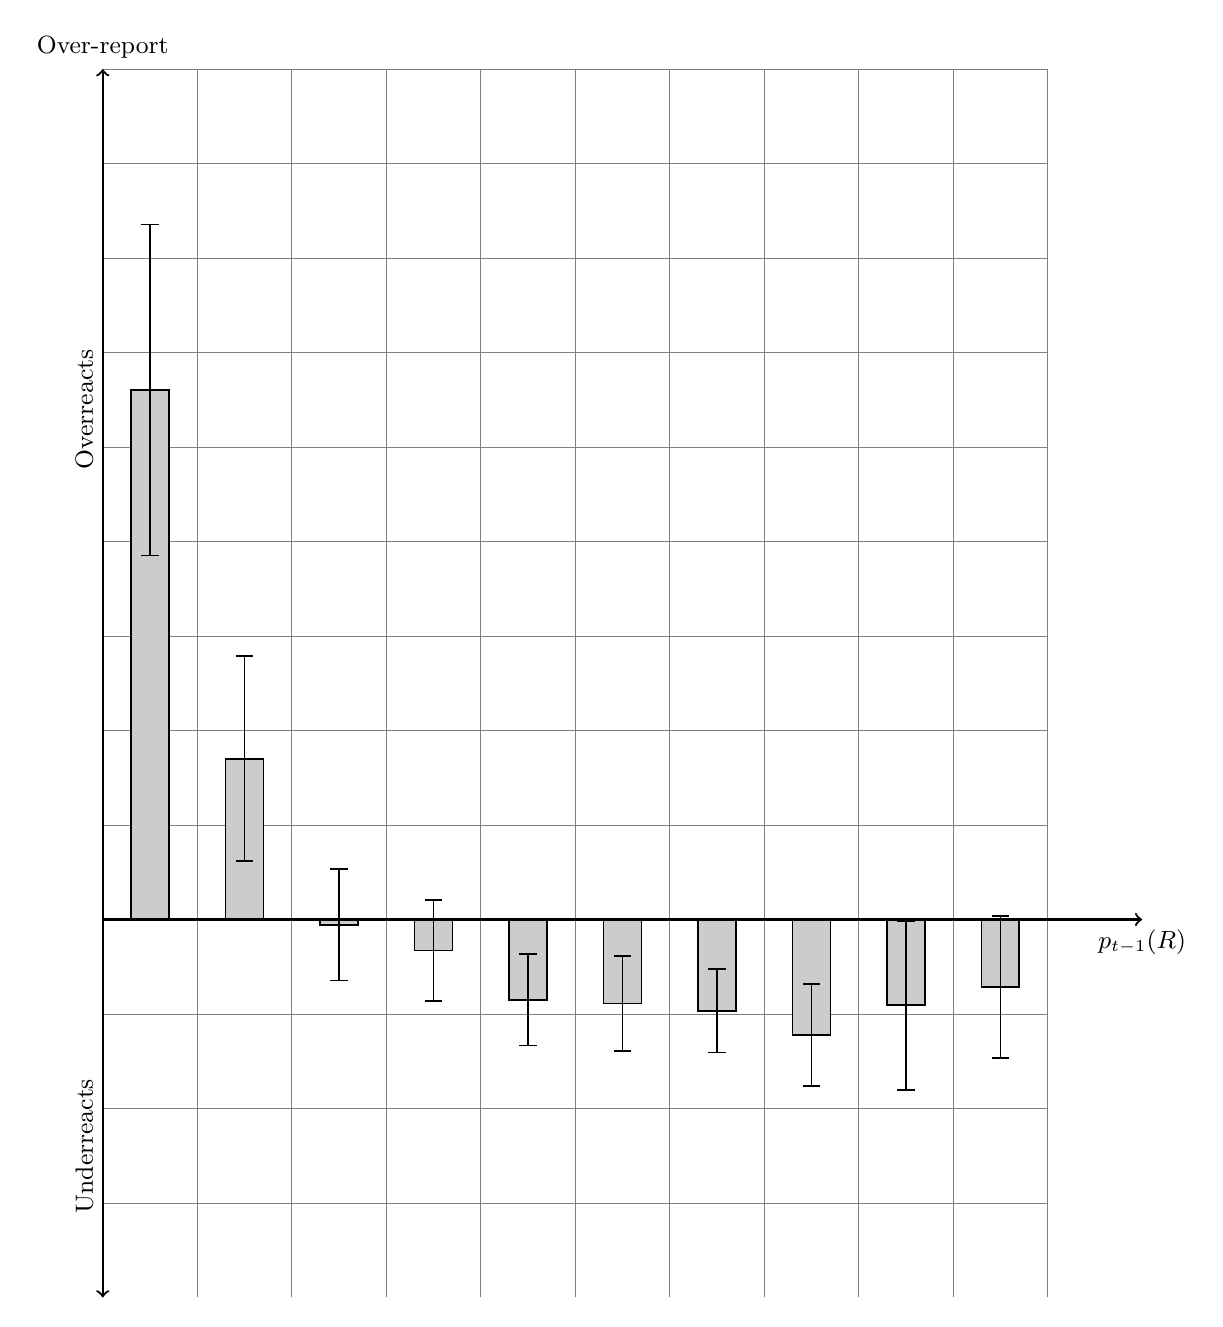
\begin{tikzpicture}[scale=12]
\draw[help lines,step=0.1] (0,-0.4) grid (1,0.9);
\filldraw[opaque,white!80!black] (0.03,0) rectangle (0.07,0.5604);
\draw[line width=0.6] (0.03,0) rectangle (0.07,0.5604);
\draw[line width=0.6,|-|] (0.05,0.3844) -- (0.05,0.7365);
\filldraw[opaque,white!80!black] (0.13,0) rectangle (0.17,0.1701);
\draw[line width=0.6] (0.13,0) rectangle (0.17,0.1701);
\draw[line width=0.6,|-|] (0.15,0.0608) -- (0.15,0.2794);
\filldraw[opaque,white!80!black] (0.23,0) rectangle (0.27,-0.0056);
\draw[line width=0.6] (0.23,0) rectangle (0.27,-0.0056);
\draw[line width=0.6,|-|] (0.25,-0.0655) -- (0.25,0.0544);
\filldraw[opaque,white!80!black] (0.33,0) rectangle (0.37,-0.0329);
\draw[line width=0.6] (0.33,0) rectangle (0.37,-0.0329);
\draw[line width=0.6,|-|] (0.35,-0.0871) -- (0.35,0.0213);
\filldraw[opaque,white!80!black] (0.43,0) rectangle (0.47,-0.0850);
\draw[line width=0.6] (0.43,0) rectangle (0.47,-0.0850);
\draw[line width=0.6,|-|] (0.45,-0.1344) -- (0.45,-0.0355);
\filldraw[opaque,white!80!black] (0.53,0) rectangle (0.57,-0.0891);
\draw[line width=0.6] (0.53,0) rectangle (0.57,-0.0891);
\draw[line width=0.6,|-|] (0.55,-0.1403) -- (0.55,-0.0379);
\filldraw[opaque,white!80!black] (0.63,0) rectangle (0.67,-0.0966);
\draw[line width=0.6] (0.63,0) rectangle (0.67,-0.0966);
\draw[line width=0.6,|-|] (0.65,-0.1415) -- (0.65,-0.0516);
\filldraw[opaque,white!80!black] (0.73,0) rectangle (0.77,-0.1223);
\draw[line width=0.6] (0.73,0) rectangle (0.77,-0.1223);
\draw[line width=0.6,|-|] (0.75,-0.1774) -- (0.75,-0.0673);
\filldraw[opaque,white!80!black] (0.83,0) rectangle (0.87,-0.0908);
\draw[line width=0.6] (0.83,0) rectangle (0.87,-0.0908);
\draw[line width=0.6,|-|] (0.85,-0.1811) -- (0.85,-0.0005);
\filldraw[opaque,white!80!black] (0.93,0) rectangle (0.97,-0.0715);
\draw[line width=0.6] (0.93,0) rectangle (0.97,-0.0715);
\draw[line width=0.6,|-|] (0.95,-0.1477) -- (0.95,0.0047);
\draw[line width=0.8,->]  (0,0) -- (1.1,0) node[below] {\small{$p_{t-1}(R)$}};
\draw[line width=0.8,<->] (0,-0.4) -- (0,0.9) node[above] {\small{Over-report}};
\draw (0,0.54) node[above,rotate=90] {\small{Overreacts}};
\draw (0,-0.24) node[above,rotate=90] {\small{Underreacts}};
% ADD THEORY CURVE BELOW
\end{tikzpicture}
